\chapter{Случайные блуждания с затуханием}
\label{ch:chap4}

\subsection*{2. Математическое ожидание}
Рекурсивное выражение:
\[
\mathbb{E}[\xi[n]] = a \, \mathbb{E}[\xi[n-1]] + \mu
\]

Решение рекурсии:
\[
\mathbb{E}[\xi[n]] = a^n \, \mathbb{E}[\xi[0]] + \mu \sum_{k=0}^{n-1} a^k
= a^n \, \mathbb{E}[\xi[0]] + \frac{\mu (1 - a^n)}{1 - a}
\]

Стационарное значение при \(n \to \infty\):
\[
\lim_{n \to \infty} \mathbb{E}[\xi[n]] = \frac{\mu}{1 - a}
\]

\subsection*{3. Дисперсия}
Рекурсивное выражение:
\[
\mathrm{Var}[\xi[n]] = \mathrm{Var}[a \,\xi[n-1] + \omega[n]] = a^2 \, \mathrm{Var}[\xi[n-1]] + \sigma^2
\]

Стационарная дисперсия при \(n \to \infty\):
\[
\sigma_\xi^2 = \frac{\sigma^2}{1 - a^2}
\]

\subsection*{4. Автокорреляционная функция}
\[
r_\xi(l) = \mathrm{E}[\xi[n] \, \xi[n-l]] = \sigma_\xi^2 \, a^{|l|}, \quad |l| \ge 0
\]

\subsection*{5. Стационарность}
Процесс стационарен в широком смысле, так как при \(n \to \infty\):
\[
\begin{aligned}
\mathbb{E}[\xi[n]] &= \frac{\mu}{1 - a}, \\
\mathrm{Var}[\xi[n]] &= \frac{\sigma^2}{1 - a^2}, \\
r_\xi(l) &= \sigma_\xi^2 \, a^{|l|}.
\end{aligned}
\]

\subsection*{Реализация}

\begin{figure}[H]
    \centering
    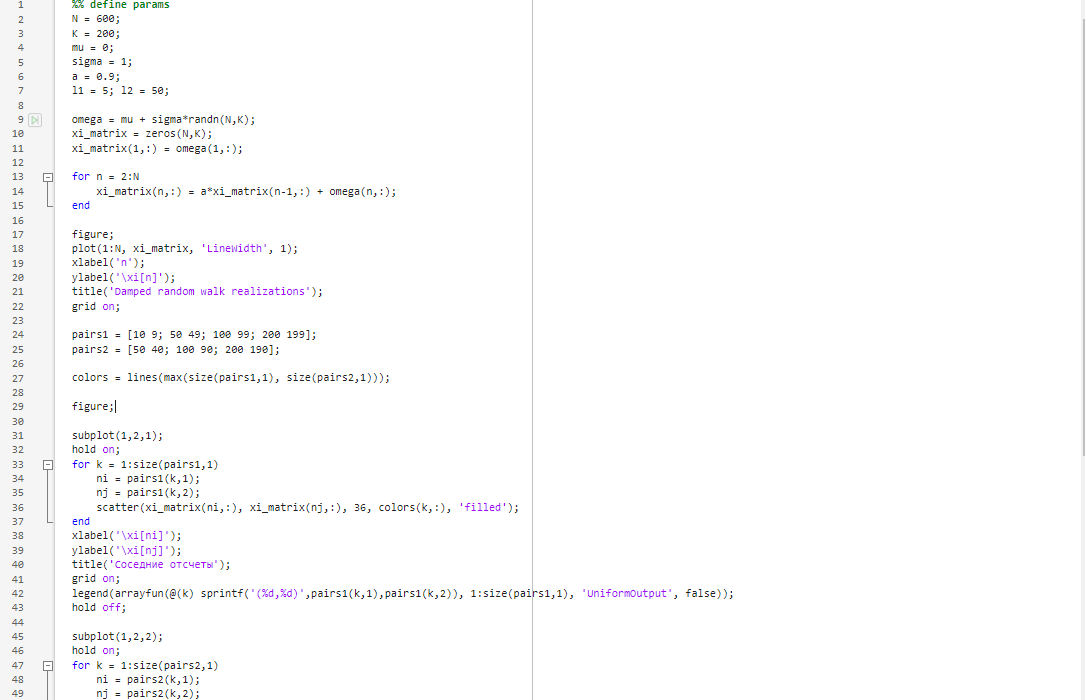
\includegraphics[width=1.0\textwidth]{drw_real1.png}
    \caption{Реализация задания с затухающим случайным блужданием}
\end{figure}

\begin{figure}[H]
    \centering
    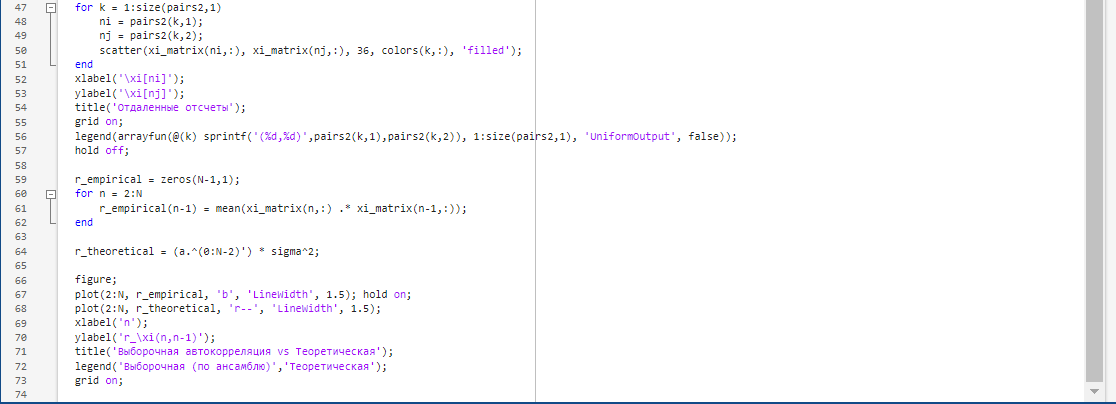
\includegraphics[width=1.0\textwidth]{drw_real_2.png}
    \caption{Реализация задания с затухающим случайным блужданием}
\end{figure}

\subsection*{Результат}

\begin{figure}[H]
    \centering
    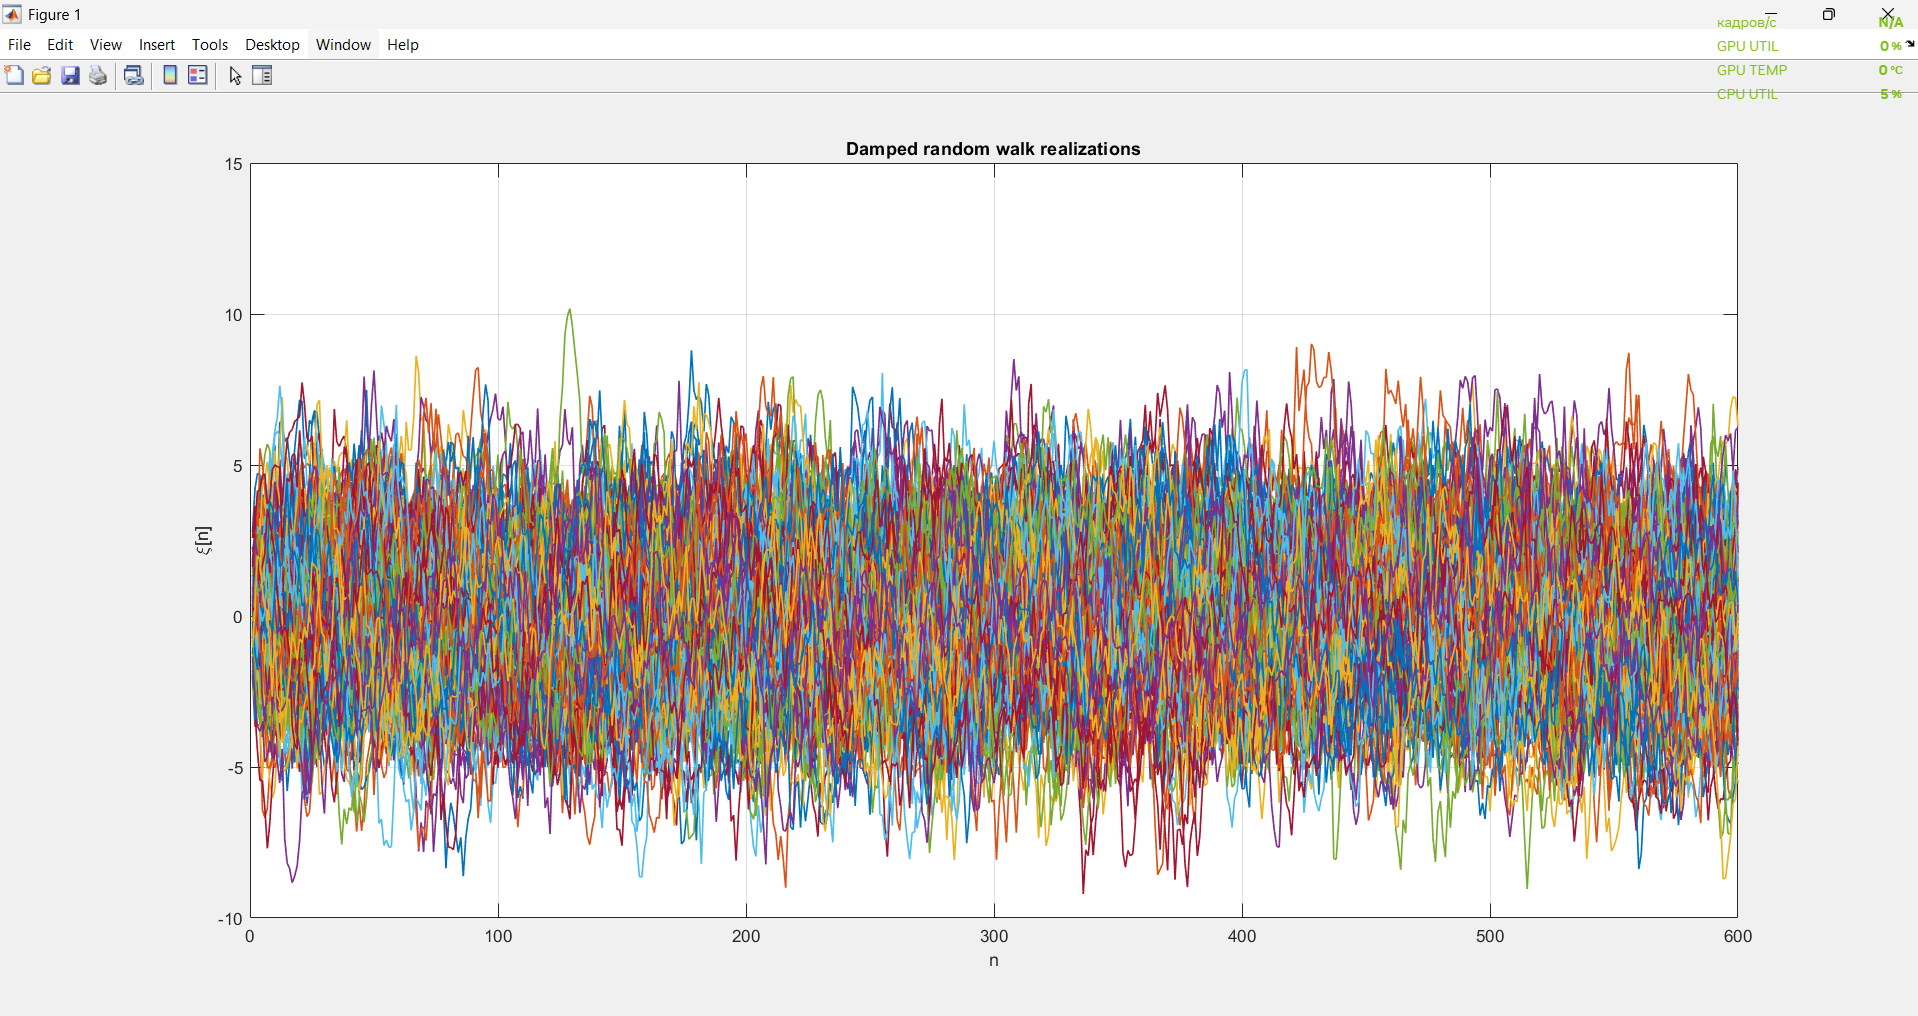
\includegraphics[width=1.0\textwidth]{dumped rw.png}
    \caption{Визуализация затухающего случайного блуждания}
\end{figure}

\begin{figure}[H]
    \centering
    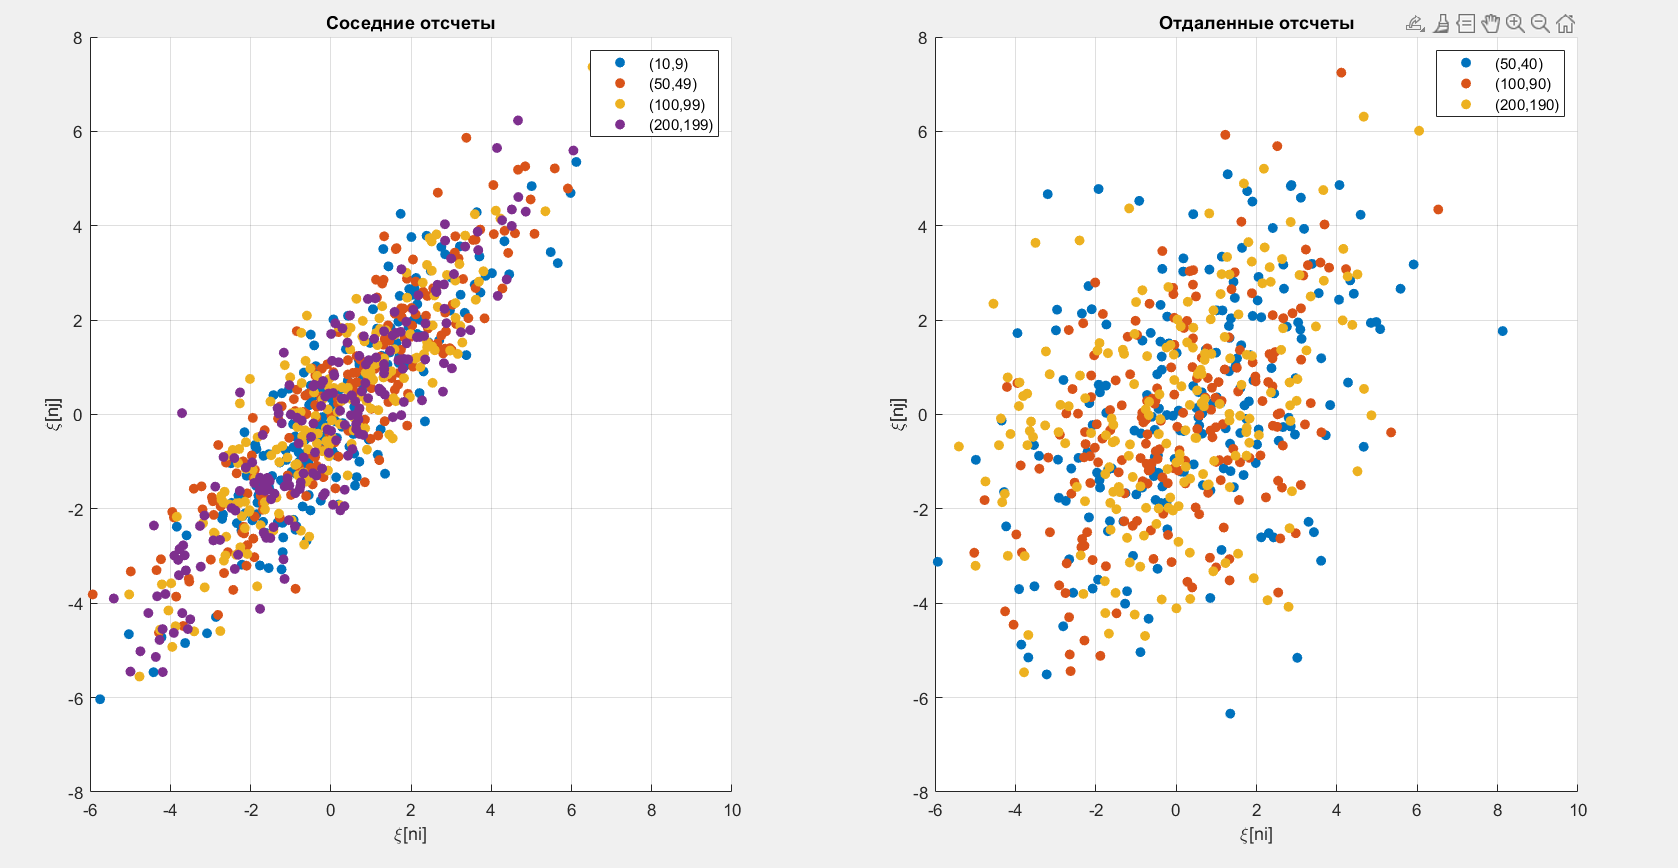
\includegraphics[width=1.0\textwidth]{drw scat.png}
    \caption{Диаграмма рассеяния затухающего случайного блуждания}
\end{figure}

\endinput